\chapter{Himmelsmechanik}
\section{Kinematik}
\subsection*{vor Newton}
\begin{description}
    \item[Aufgabe] genaue Beschreibung der scheinbaren Bewengung
        \begin{itemize}
            \item \emph{nicht} die Erklärung/das Verständnis des zugrunde
                  liegenden Sachverhaltes (Gesetztes)
        \end{itemize}
    \item[speziell] scheinbare Planetenbahnen $\rightarrow$ Mars
        \begin{center}
            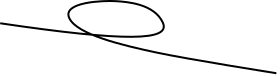
\includegraphics[width=.3\textwidth]{img/ptolemaeus_mars.pdf}
        \end{center}
    \item[Modelle]
        \begin{itemize}
            \item \textsc{Ptolemäus:}
                \begin{itemize}
                    \item Geozentrisch (Erde im Zentrum)
                    \item Planeten auf Epizykelbahnen
                \end{itemize}
            \item \textsc{Kopernikus:}
                \begin{itemize}
                    \item Heliozentrisch (Sonne im Zentrum)
                    \item \emph{Kreisbahnen}
                \end{itemize}
        \end{itemize}
    \item[Enscheidung] z. B. Planetenphasen der inneren Planeten\\
        $\Rightarrow$ Kopernisches Weltbild
\end{description}
\begin{itemize}
    \item \textsc{Kepler:} Messung d. Marsbahnen (T. \textsc{Brahe})\\
          $\Rightarrow$ \textsc{Kepler}'sche Gesetze (empirisch)
          \begin{enumerate}
              \item Ellipsen, Sonne in einem Brennpunkt
              \item Flächensatz $\Leftrightarrow$ Drehimpulserhaltung \\
                    Radiusvektoren überstreichen in gleicher Zeit gleiche Flächen,\\
                    d. h. Flächengeschwindigkeit = $\mathbf{const}$
              \item Umlaufzeiten/Abstände ($a$: Halbachse, $T$: Umlaufzeit)
                      \[ \frac{a^3}{T^2} \sim \mathbf{const} \]
          \end{enumerate}
\end{itemize}

\section{Newton'sche Mechanik}
\textsc{Newton}'sche Axiome:
\begin{enumerate}[(i)]
    \item Trägheitsgesetz (Masse konstant, vergl. spezielle Relativitätstheorie):
        \[ \vec p = m \vec v = m \dot{\vec{r}} = m \frac{d}{dt} \vec r \]
    \item Impulsänderung durch Krafteinwirkung:
        \[ \frac{d}{dt} \vec p = \dot{\vec p} = \vec F = m \ddot{\vec r} = m \frac{d^2}{dt^2} \vec r = m \vec a \]
    \item Actio = Reactio:
        \[ \vec F_{ik} = -\vec F_{ki} \]
\end{enumerate}
